\input{../header_common.tex}

\subject{V103}
\title{Biegung elastischer Stäbe}
\author{Nicolai Weitkemper \and Katharina Popp}
\date{
    Durchführung: 24.11.2020
    \hspace{3em}
    Abgabe: 08.11.2020
}

\begin{document}

\maketitle
\thispagestyle{empty}
\tableofcontents
\newpage


\section{Zielsetzung} \label{sec:Ziel}

    Im Folgenden Versuch soll das Elastizitätsmodul von Metallproben in Form von
    Stäben mithilfe von elastischer Biegung bestimmt werden.

\section{Theorie} \label{sec:theorie}

\subsection{Problemstellung} \label{sec:problem}

    Die Kraft $F$, die auf eine Fläche wirkt, wird als Spannung bezeichnet.
    Man unterscheidet zwischen der senkrecht wirkenden Komponente, der Normalspannung $\sigma$,
    und der parallel zur Fläche wirkenden Komponente, der Tangential- oder Schubspannung.
    Die Normalspannung ist proportional zur Längenänderung $\symup{\Delta}L$ und wird
    durch das Hookesche Gesetz beschrieben:
    \begin{equation}
        \sigma = E \cdot \frac{\symup{\Delta}L}{L} .
    \end{equation}
    Das Elastizitätsmodul $E$ stellt eine wichtige Materialkonstante eines Stoffes dar und 
    ist hier ein Proportionalitätsfaktor.
    Diese Größe kann mithilfe der Biegung eines Körpers bestimmt werden, 
    wobei die Durchbiegung durch eine Funktion $D(x)$ beschrieben wird.
    $D(x)$ setzt sich aus der Auslenkung $D_0(x)$ bei einer sogenannten Nullmessung, 
    einer Messung ohne angehängtes Gewicht, und einer Auslenkung $D_\text{M}(x)$  bei einer
    Messung mit angehängtem Gewicht zusammen.
    Es gilt
    \begin{equation}
        D(x) = D_\text{M}(x) - D_0(x) .
    \end{equation}

    Im Folgenden sollen zwei Möglichkeiten zur Berechnung der Biegung vorgestellt werden.

\subsection{Durchbiegung eines homogenen Stabes bei einseitiger Einspannung} \label{sec:einseitig}

    Die erste Möglichkeit besteht darin, einen Stab an einer Seite einzuspannen.
    Die Funktion $D(x)$ kann durch ein Drehmoment $M_\text{F}$ berechnet werden, welches die anliegende Kraft F erzeugt.
    Das Drehmoment bewirkt eine Änderung des Querschnitts des Stabes. Die oberen Schichten werden gedehnt und die unteren
    gestaucht. Dazwischen liegt die neutrale Faser, eine Fläche, die ihre ursprüngliche Länge beibehält.
    Im Inneren treten Normalspannungen auf, die ein inneres Drehmoment $M_{\symup{\sigma}}$ erzeugen. 
    Der Stab wird soweit gebogen, bis das äußere und innere Drehmoment gleich sind: 
    \begin{equation}
        M_{\symup{\sigma}} = M_\text{F}
    \end{equation}
    mit 
    \begin{equation}
        M_{\symup{\sigma}} = \int_Q y\sigma(y) dq 
    \end{equation}
    und
    \begin{equation}
        M_\text{F} = F (L-x) .
    \end{equation}
    Die Variable $x$ stellt eine beliebige Stelle auf dem Stab dar, $Q$ ist der Querschnitt des Stabes und $y$ beschreibt den 
    Abstand zwischen Flächenelement dq und der neutralen Faser.
    Für $D(x)$ ergibt sich 
    \begin{equation}
        D(x) = \frac{F}{2EI} \left(Lx^2 - \frac{x^3}{3}\right) \label{eqn:einsD}
    \end{equation}
    für $0 \leq x \leq L$. Die Variable $I$ stellt das Flächenträgheitsmoment dar.

\subsection{Durchbiegung eines homogenen Stabes bei beidseitiger Einspannung} \label{sec:beidseitig}

    Die zweite Möglichkeit besteht darin, den Stab an beiden Enden einzuspannen und die Kraft in der 
    Mitte des Stabes angreifen zu lassen.
    Für das äußere Drehmoment $M_\text{F}$ ergibt sich 
    \begin{equation}
        M_\text{F} = - \frac{F}{2} x 
    \end{equation}
    für $0 \leq x \leq \frac{L}{2}$ und
    \begin{equation}
        M_\text{F} = \frac{F}{2} (L-x)
    \end{equation}
    für $\frac{L}{2} \leq x \leq L$.
    Für $D(x)$ ergibt sich 
    \begin{equation}
        D(x) = \frac{F}{48EI} (3L^2 x - 4x^3) \label{eqn:beidD1}
    \end{equation}
    für $0 \leq x \leq \frac{L}{2}$ und 
    \begin{equation}
        D(x) = \frac{F}{48EI} (4x^3 - 12Lx^2 + 9L^2 x - L^3) \label{eqn:beidD2}
    \end{equation}
    für $\frac{L}{2} \leq x \leq L$. \\ \\ \\

Das Elastizitätsmodul kann durch Umformen der Gleichungen \eqref{eqn:einsD} , \eqref{eqn:beidD1} oder \eqref{eqn:beidD2}
für den jeweiligen Fall berechnet werden.
\newpage

\section{Durchführung}
\label{sec:durchfuehrung}

    Der folgende Abschnitt beinhaltet die Durchführung der verschiedenen Messungen.

\subsection{Messung einer Entladekurve des Kondensators}

    Für die Bestimmung der Zeitkonstante $RC$ kann entweder die Entlade- oder die Aufladekurve des Kondensators untersucht werden.
    Hier wird die Entladekurve gemessen,
    wobei die verwendete Schaltung in der folgenden Abbildung \ref{fig:messung_entladekurve} dargestellt ist.

    \begin{figure}
        \centering
        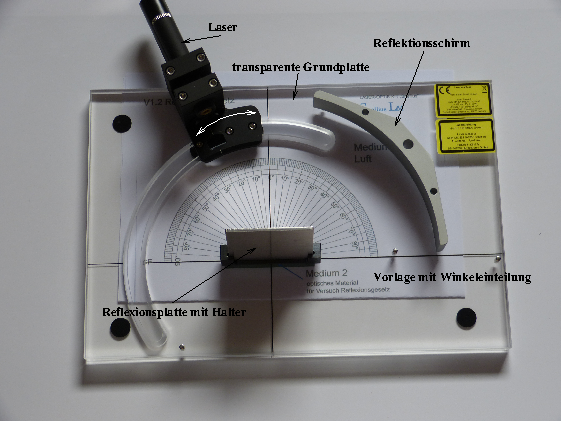
\includegraphics{content/img/Abb_3.pdf}
        \caption{Schaltung zur Messung der Auf- und Entaldekurve des Kondensators im RC-Kreis.}
        \label{fig:messung_entladekurve}
    \end{figure}

    Zu Beginn der Messung muss an Generator eine Rechteckspannung eingestellt werden,
    welche auf einem Oszilloskop in Abhängigkeit von der Zeit darstellbar ist.
    Die Entladekurve ist in Abbildung \ref{fig:entladekurve} zu sehen.

    \begin{figure}
        \centering
        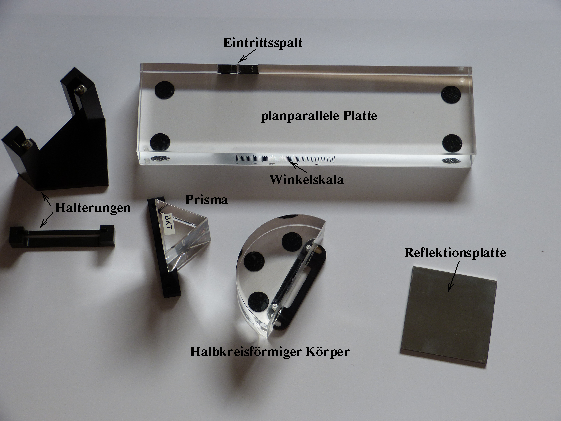
\includegraphics{content/img/Abb_4.pdf}
        \caption{Gestalt der Entladekurve.}
        \label{fig:entladekurve}
    \end{figure}

    Es werden fünfzehn Messwerte aufgenommen,
    wobei die Zeitkonstante mithilfe der Gleichung \eqref{eqn:entladung} berechnet werden kann.

\subsection{Messung der Amplitude und der Phasenverschiebung}

    Für diese Messung wird am Generator eine Sinusförmige Spannung angelegt,
    welche wieder auf einem Oszilloskop dargestellt werden kann.\\
    Für die Messung der Amplitude wird die folgende Schaltung verwendet.

    \begin{figure}
        \centering
        \includegraphics{content/img/Abb_5.pdf}
        \caption{Schaltung zur Messung der Spannungsamplitude in Abhängigkeit der Frequenz.}
        \label{fig:messung_amplitude}
    \end{figure}

    Zu Beginn wird die Frequenz der kleinst- und größtmöglich darstellbaren Amplitude bestimmt,
    in diesem Fall lag die größtmögliche Amplitude bei $\omega = \SI{10}{\hertz}$ und die kleinstmögliche Amplitude bei $\omega = \SI{2000}{\hertz}$.
    Anschließend wird das Intervall zwischen beiden Frequenzwerten in geeigneten Abständen ausgemessen.
    Die Zeitkonstante kann mit Umstellen der Gleichung \eqref{eqn:amplitude} berechnet werden.\\
    \\
    Die Messung der Phasenverschiebung kann mit denselben Einstellungen durchgeführt werden.

    \begin{figure}
        \centering
        \includegraphics{content/img/Abb_6.pdf}
        \caption{Schaltung zur Messung der Phasenverschiebung von Generatr- und Kondensatorspannung.}
        \label{fig:messung_phasenverschiebung}
    \end{figure}

    In Abbildung \ref{fig:messung_phasenverschiebung} ist die verwendete Schaltung gezeigt.
    Die Generatorspannung $U_\text{G}$ wird am Eingang $Y_\text{A}$ angeschlossen,
    die Kondensatorspannung $U_\text{C}$ am Eingang $Y_\text{B}$.
    Am Oszilloskop muss die Einstellung \textit{DUAL} ausgewählt werden,
    um gleichzeitig die eingehende Generatorspannung und die Kondensatorspannung zu sehen.
    Es wird dasselbe Frequenzintervall wie vorher abgelaufen,
    wobei die Abstände $a$ und $b$ entsprechend der Darstellung in Abbildung \ref{fig:phasenverschiebung} gemessen werden.

    \begin{figure}
        \centering
        \includegraphics{content/img/Abb_7_edit.pdf}
        \caption{Die Phasenverschiebung zwischen Generatorspannung und Kondensatorspannung.}
        \label{fig:phasenverschiebung}
    \end{figure}

    Die Phasenverschiebung kann mithilfe von
    \begin{align*}
        \phi &= \frac{a}{b} \cdot 360 & \phi &= \frac{a}{b} \cdot 2 \symup{\pi}
    \end{align*}
    bestimmt und in Gleichung \eqref{eqn:phasenverschiebung} zur Berechnung der Zeitkonstante eingesetzt werden.

\newpage

\section{Auswertung} \label{sec:Auswertung}

In \autoref{tab:messwerte} sind sämtliche zur Verfügung gestellten Messwerte aufgelistet.
Der (gerundete) Fehler der Zählrate $Z$, der sich aus $\sqrt{N}$ berechnet, wurde ebenfalls angegeben.
Die Ablesegenauigkeit des Amperemeters ist konstant $\symup{\Delta}I=\SI{0.05}{\micro\ampere}$.

\begin{table}[H]
  \centering
  \caption{Übersicht aller aufgenommenen Messwerte.}
  \label{tab:messwerte}
  \begin{tabular}{c c c}
  \toprule
  $U \mathbin{/} \si{\volt}$ &
  $N \mathbin{/} \si{{Imp} \per 60 \second}$ &
  $I \mathbin{/} \si{\micro\ampere}$ \\
  \midrule
  \expandableinput{build/table_messwerte.tex}
  \bottomrule
  \end{tabular}
\end{table}


\subsection{Aufnahme der Geiger-Müller-Charakteristik}

% Die Integrationszeit pro Zählrohrspannung betrug t = 60s, damit die Zählrate
% im Geiger-Plateau in der Größenordnung von N = 10000 Imp liegt. (Warum? Begründung
% nicht vergessen)

\begin{figure}
  \centering
  \includegraphics[width=\textwidth]{build/plot1.pdf}
  \caption{Impulsrate in Abhängigkeit der Spannung.}
  \label{fig:plot1}
\end{figure}

Weil die Zählraten Poisson-verteilt sind, sind die Messunsicherheiten durch $\symup{\Delta}N = \sqrt{N}$ gegeben.
Das Plateau liegt in etwa zwischen $\SI{370}{\volt}$ und $\SI{640}{\volt}$
und ist in \autoref{fig:plot1} durch gestrichelte Linien begrenzt.
% /gekennzeichnet
Die Plateaulänge beträgt also ungefähr $\SI{270}{\volt}$.
Für diesen Bereich wurde
der Plateauanstieg durch
eine Regressionsgerade
zu $\SI{19.198(3727)}{{Imp}\per\second\per\kilo\volt}$
% und Achsenabschnitt
bestimmt.

\subsection{Bestimmung der Totzeit}

\subsubsection{Zwei-Quellen-Methode}
\label{sec:totzeit_zweiquellen}

Bei einer Messzeit von $t = \SI{120}{s}$ wurden folgende Zählraten gemessen:

\begin{align*}
N_{1}   &= \SI{96041} {{Imp} \per 120 \second} \\
N_{1+2} &= \SI{158479}{{Imp} \per 120 \second} \\
N_{2}   &= \SI{76518} {{Imp} \per 120 \second} \\
\end{align*}

Nach \autoref{eqn:totzeit} ergibt sich daraus eine Totzeit von $T \approx \SI{115(4)}{\micro\second}$.
Die Messunsicherheit
% welche auch nach der Gaußschen Fehlerfortpflanzung bestimmbar wäre,
wurde mit dem Python-Paket \textit{uncertainties} berechnet.

% Der Fehler kann gemäß der Gaußschen Fehlerfortpflanzung folgendermaßen berechnet werden:
% \begin{equation*}
%   \symup{\Delta}T =
%   \frac{N_{1+2}-N_2}{2N_1^2N_2} \cdot \symup{\Delta}N_1 +
%   \frac{N_{1+2}-N_1}{2N_2^2N_1} \cdot \symup{\Delta}N_2 -
%   \frac{1}{2N_1N_2} \cdot \symup{\Delta}N_{1+2}
% \end{equation*}


\subsubsection{Oszilloskop}
\label{sec:totzeit_oszilloskop}

Die Zeitachse am Oszilloskop bemisst sich auf $\SI{100}{\micro\second \per {DIV}}$,
sodass jeder Strich $\SI{20}{\micro\second \per {DIV}}$ entspricht.

Es wurde nun die Totzeit als Zeit zwischen dem ersten und zweiten Puls abgelesen,
wie in \autoref{fig:totzeit_oszilloskop} dargestellt ist.
Diese ergab sich zu $T \approx \SI{110(20)}{\micro\second}$,
wobei die Unsicherheit als der Abstand zwischen zwei Strichen abgeschätzt ist.

\begin{figure}[H]
  \centering
  \includegraphics[width=0.75\textwidth]{content/img/totzeit_oszilloskop.jpg}
  \caption{Momentaufnahme des Oszilloskops mit eingezeichneten Extrema und Zeiten \cite{oszilloskop}.}
  \label{fig:totzeit_oszilloskop}
\end{figure}

% In DatenHinweiseGeigerMueller.pdf steht: Bestimmung des Zählrohrstroms 🤔
\subsection{Bestimmung der pro Teilchen freigesetzten Ladungen}

Gemäß \autoref{eqn:Teilchenzahl} lässt sich aus der Anzahl eingefallener Teilchen und dem Zählerstrom
auf die Anzahl der freigesetzten Ladungen pro einfallendem Teilchen schließen.
In \autoref{fig:plot2} ist dieses Verhältnis gegen die anliegende Spannung aufgetragen.
Die Messunsicherheit wurde wieder mit \textit{uncertainties} berechnet.

Im Mittel ergibt sich $Z=\num{3.43(6)e+10}$.

\begin{table}[H]
  \sisetup{separate-uncertainty=true}
  \centering
  \caption{Zahl der pro einfallendem Teilchen freigesetzten Ladungen.}
  % \label{tab:messwerte}
  \begin{tabular}{c c c c}
  \toprule
  $U \mathbin{/} \si{\volt}$ &
  $N \mathbin{/} \si{{Imp} \per 120 \second}$ &
  $I \mathbin{/} \si{\micro\ampere}$ &
  $Z [10^{10}]$ \\
  \midrule
  \expandableinput{build/table_zaehlrohrstrom.tex}
  \bottomrule
  \end{tabular}
\end{table}

\begin{figure}[H]
  \centering
  \includegraphics[width=\textwidth]{build/plot2.pdf}
  \caption{Zahl der freigesetzten Ladungen pro eingefallenem Teilchen in Abhängigkeit der Spannung.}
  \label{fig:plot2}
\end{figure}


\end{document}